\documentclass[spanish,12pt,a4paper,titlepage]{report}
\usepackage[utf8]{inputenc}
\usepackage{graphicx}
\usepackage{subfig}
\usepackage{float}
\usepackage{wrapfig}
\usepackage{multirow}
\usepackage{caption}
\usepackage[spanish]{babel}
\usepackage[dvips]{hyperref}
\usepackage{amssymb}
\usepackage{listings}
\usepackage{epsfig}
\usepackage{amsmath}
\usepackage{array}
\usepackage[table]{xcolor}
\usepackage{multirow}
%\usepackage[Sonny]{fncychap}
\usepackage[Lenny]{fncychap}
%\usepackage[Glenn]{fncychap}
%\usepackage[Conny]{fncychap}
%\usepackage[Rejne]{fncychap}
%\usepackage[Bjarne]{fncychap}
%\usepackage[Bjornstrup]{fncychap}

%\usepackage{subfiles}
%\usepackage{framed}

\setlength{\topmargin}{-1.5cm}
\setlength{\textheight}{25cm}
\setlength{\oddsidemargin}{0.3cm} 
\setlength{\textwidth}{15cm}
\setlength{\columnsep}{0cm}



\newcommand{\HRule}{\rule{\linewidth}{0.5mm}}
\begin{document}

\chapter{Calibración de giróscopo}

\section{Objetivos}

\begin{itemize}
	\item Realizar una serie de pruebas con el fin de calibrar el giróscopo de tres ejes de la IMU.
	\item Estudiar, proponer y validar un modelo posible para dicha calibración.
	\item Estimar las fuentes de error del mismo (ruido y bias).
\end{itemize}

\section{Materiales}
\begin{itemize}
\item Mongoose 9Dof IMU de \emph{Ckdevices}
\item Beagleboard xM
\item Adaptador Wi-Fi 
\item Tocadiscos
\item Cronómetro
\item Cubo perfecto de madera
\item 2 escuadras de 45º
\item 2 escuadras de 30º
\item Madera de 4 cm de ancho con lados paralelos
\end{itemize}

\section{Marco teórico}
Para la calibración del giróscopo se utiliza el mismo modelo que se utilizó para el acelerómetro en la sección \ref{chap:calibracion_acelerometro}, se estudia las no idealidades que afectan la lectura de los valores de velocidad angular registrados en el dispositivo y se validan los resultados obtenidos. Las no idealidades  a considerar basados en lo desarrollado por \cite{bib:calib_IMU} son:

\begin{itemize}
\item Ruido inherente
\item Relación entre aceleración real y lectura del acelerómetro no lineal.
\item No ortogonalidad de los ejes
\item Drift aleatorio
\item Variación de las medidas con la temperatura
\end{itemize}

El modelo para la calibración del giróscopo, como puede verse con más detalle en el capítulo \ref{chap:calibracion_acelerometro}, es:
$$\tilde{\mathbf{w^a}}=K_w(T_a^p)^{-1}\mathbf{w^p}+b_w$$
con $K_w$ matriz diagonal que representa el factor de escala para convertir del valor digital a la aceleración correspondiente, $\mathbf{b}_w$ un término independiente para corregir la posición del cero y $T^p_a$ una matriz que corrige la no perpendicularidad perfecta de los ejes:
$$T^p_a=\left( 
\begin{matrix}
1 &-\alpha_{yz} &\alpha_{zy}\\
\alpha_{xz} &1& -\alpha_{zx} \\
-\alpha_{xy} &\alpha_{yx} &1\\
\end{matrix} 
\right)$$

A su vez, estos parámetros varían con la temperatura, lo cual puede introducir errores significativos dependiendo del estado del tiempo, la estación del año, o la hora del día

\section{Procedimiento}
\subsection{Caracterización de las no idealidades variables}

Para obtener más información sobre el \emph{ruido inherente} y el \emph{drift aleatorio} se toman datos durante una hora a una frecuencia de 50 Hz con el dispositivo quieto.\\

\subsection{Determinación de parámetros estáticos}

Para poder realizar la calibración pertinente es necesario determinar 12 parámetros: las ganancias y bias de los 3 ejes y los 6 ángulos de la matriz $T^p_a$. Para determinar dichos parámetros es conveniente obtener el doble o triple de medidas que de parámetros. Las medidas a realizar son las siguientes:

\begin{table}[H]
\centering
\begin{small}
\begin{tabular}{|c|c|c|}
\hline
  {\cellcolor[gray]{0.85} \centering \textbf{Eje de giro principal}}
& {\cellcolor[gray]{0.85} \centering \textbf{Eje de giro secundario}}
& {\cellcolor[gray]{0.85} \centering \textbf{Ángulo de giro}} \\ \hline  \hline
x & z & 0 \\ \hline
x & z & 30 \\ \hline
x & z & 45 \\ \hline
y & x & 0 \\ \hline
y & x & 30 \\ \hline
y & x & 45 \\ \hline
z & y & 0 \\ \hline
z & y & 30 \\ \hline
z & y & 45 \\ \hline
\end{tabular}
\caption{Configuraciones utilizadas para calibrar el giróscopo}
\label{tab:gyros}
\end{small}
\end{table} 

Con un total de 9 configuraciones diferentes, donde cada una de ellas aporta 3 medidas (una por cada eje), se utilizarán un total de 27 medidas para determinar los 12 parámetros involucrados.

\subsubsection*{Preparación}

Las medidas consisten básicamente en dejar la IMU girar a la velocidad del tocadiscos en las posiciones listadas en la tabla \ref{tab:gyros}. 

\begin{wrapfigure}{l}{0.6\textwidth}
  \vspace{-20pt}
  \begin{center}
    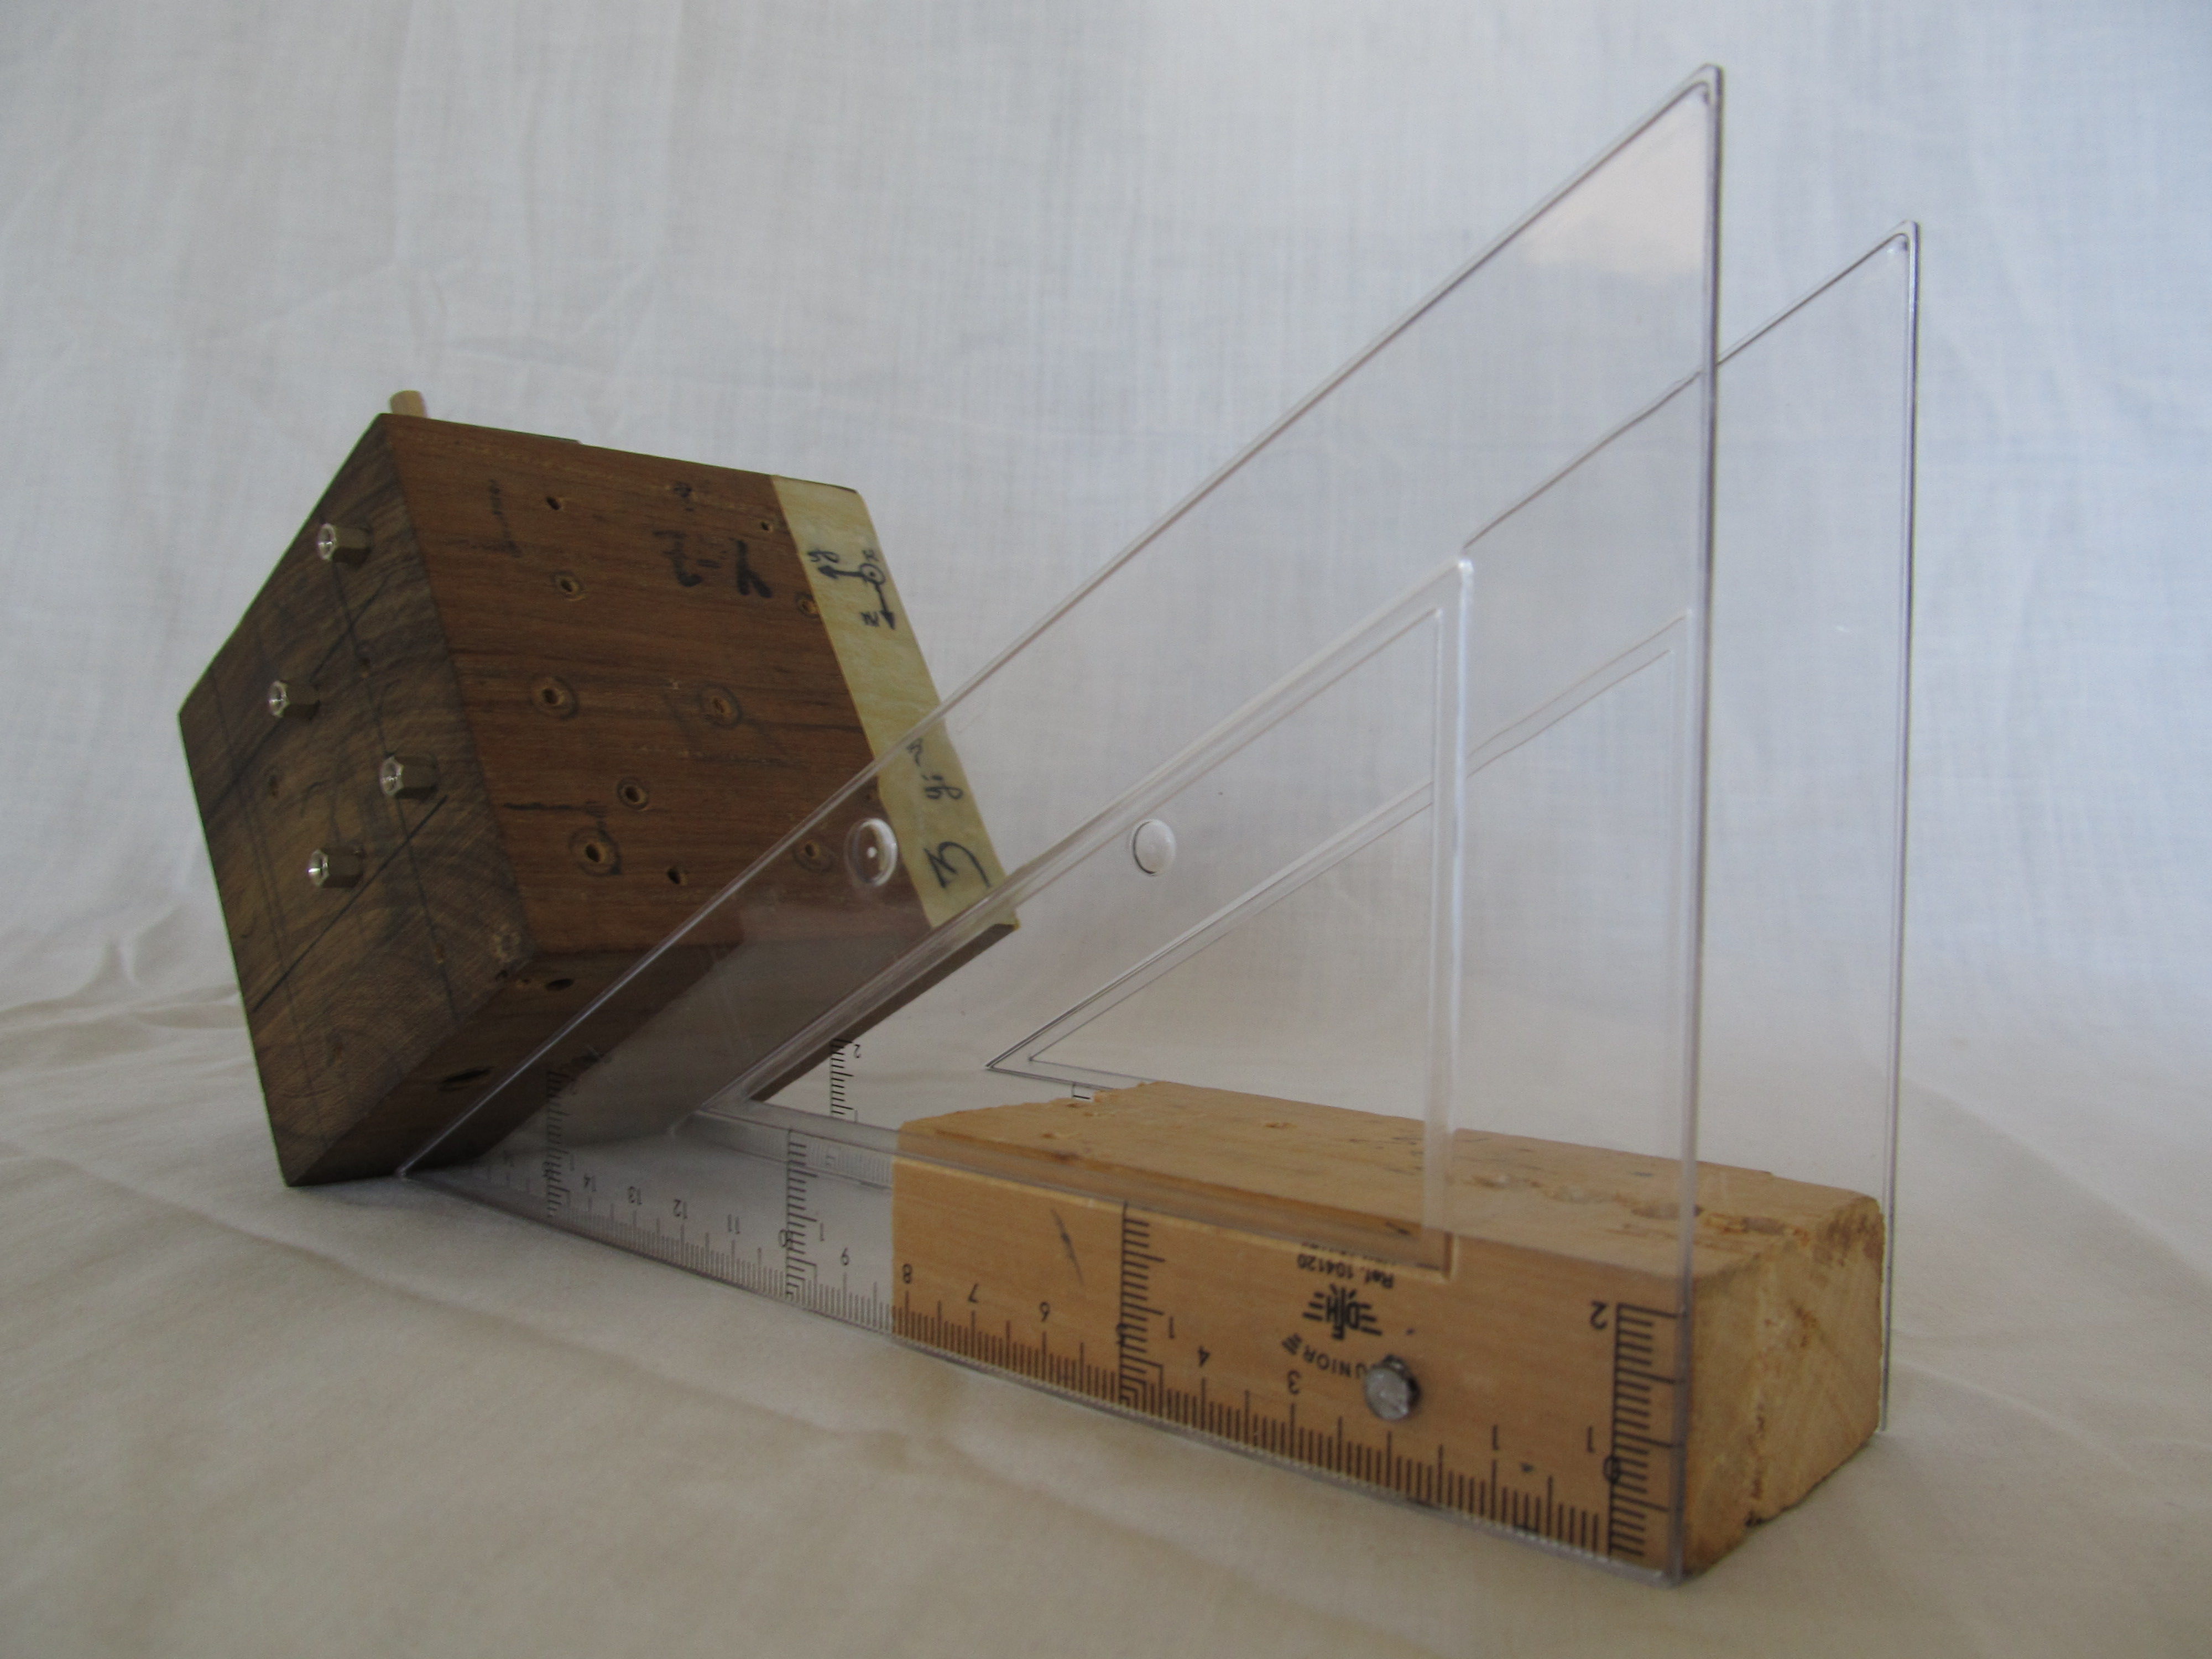
\includegraphics[width=0.45\textwidth]
    	{./pics/escuadra.jpg}
  \end{center}
  \vspace{-20pt}
  \caption{Escuadras}
  \label{fig:escuadras}
  \vspace{-10pt}
\end{wrapfigure}

La dirección de giro principal es la dirección de giro del tocadiscos cuando no hay giro en la dirección secundaria. Con el cubo de madera se resuelven las rotaciones de 90 grados para alinear los diferentes ejes de la IMU con el eje de giro del tocadiscos. Los giros en el eje secundario se realizan utilizando las escuadras y la madera de 4 cm de ancho y lados paralelos, como se muestra en la figura \ref{fig:escuadras}. Apoyando el cubo sobre la escuadra se logran los ángulos de $30º$ y $45º$ deseados en las direcciones de giro secundarias.\\

Si bien la velocidad de giro estándard del tocadiscos es 33.3 rpm, resulta conveniente medir la velocidad del tocadiscos para corroborarla. Se mide la velocidad con el dispositivo IR y se verifica el buen funcionamiento del tocadiscos.\\

Un esquema completo de la configuración utilizada para la calibración del girósopo se puede ver en la figura \ref{fig:tocadiscos}.

\begin{figure}[h!]
	\centering
	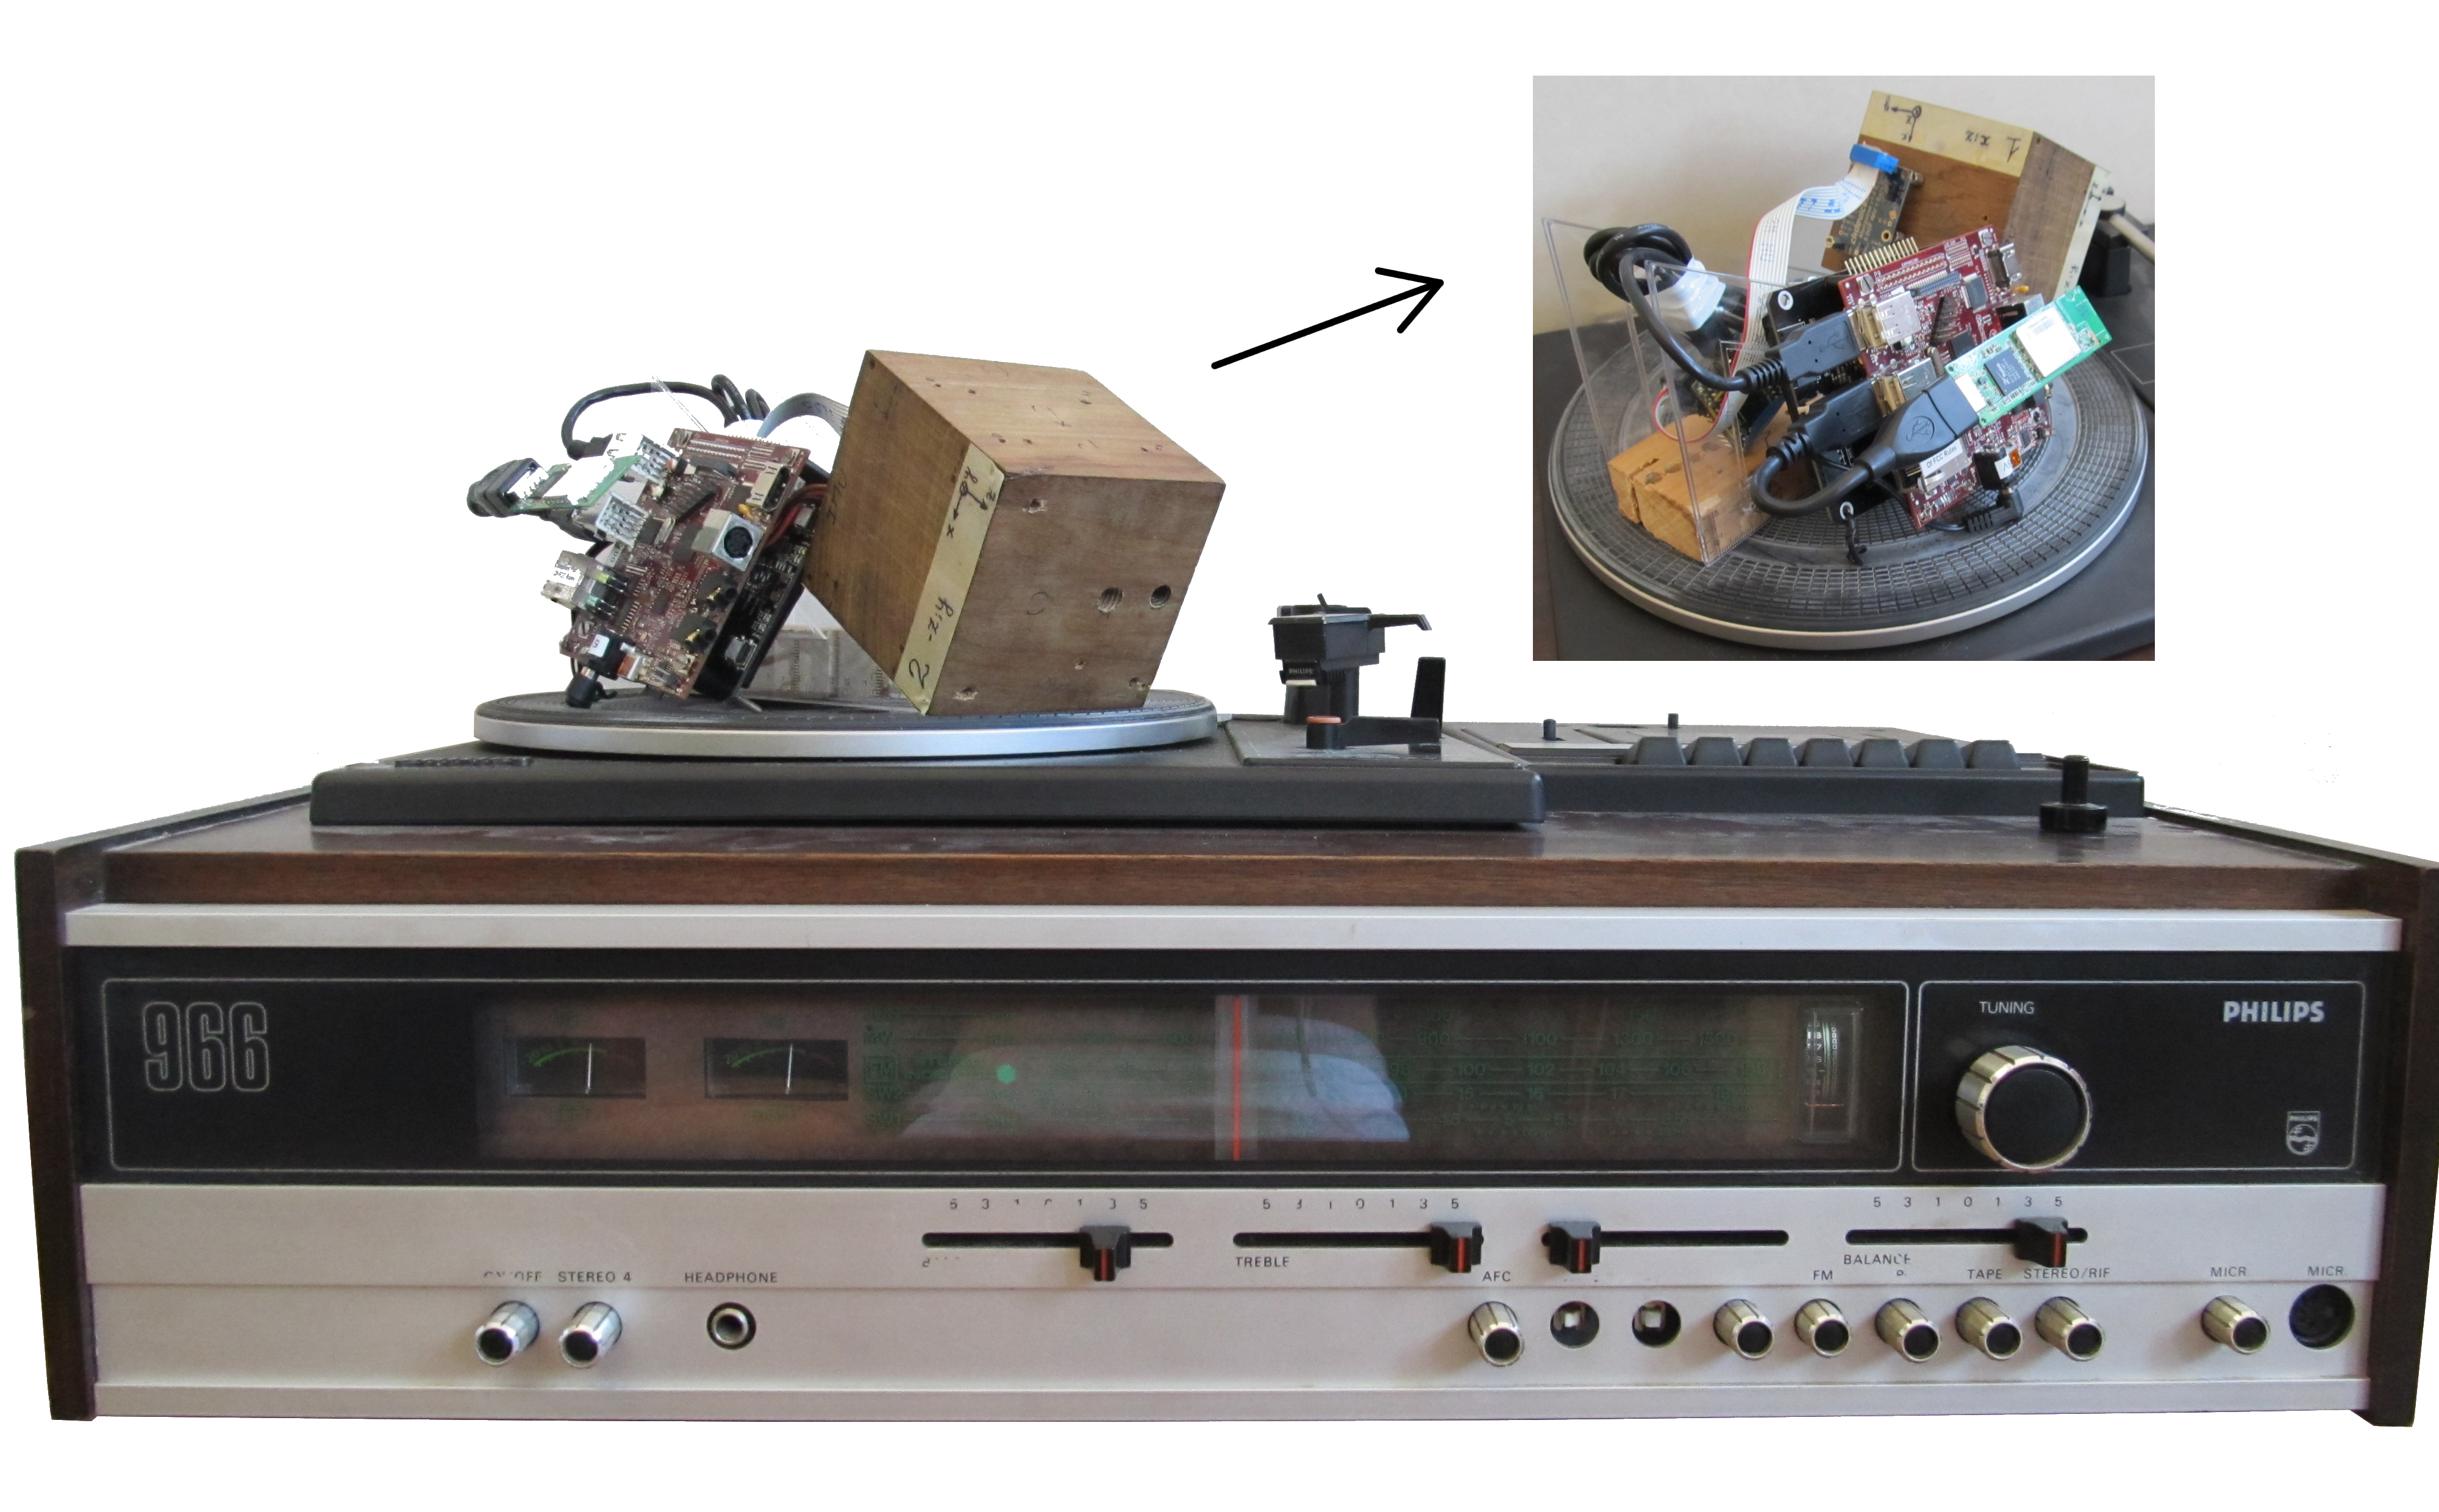
\includegraphics[width=.9\textwidth]{./pics/tocadiscos.jpg}
	\caption{Tocadiscos}
	\label{fig:tocadiscos}
\end{figure}


\section{Resultados y análisis}
\subsection{Medias estáticas para el giróscopo}
Se pone el tocadiscos a girar y mediante la conexión Wi-Fi se indica a la \emph{BeagleBoard xM} que empiece y termine de logear los datos. Se trabaja con el promedio de las velocidades angulares obtenidas en series de datos de 20 segundos controlados por cronómetro. La velocidad del tocadiscos permanece constante en todas las pruebas y lo que se varía es el ángulo del plano donde se apoya el cubo, haciendo uso de las escuadras (figura \ref{fig:escuadras}).\\

La IMU arroja datos enteros en complemento A2 convertidos a $grados/segundo$. Dicha conversión se hace internamente a la IMU utilizado la siguiente ganancia asegurada en la hoja de datos: $14.375\quad LDB/(º/s)$.\\

Al igual que con la calibración del acelerómetro (capítulo \ref{chap:calibracion_acelerometros}), se utiliza la función \emph{lsqnonlin} de \emph{Matlab} para ajustar las medidas obtenidas contra los valores teóricos para cada configuración. Dado que las medidas ya vienen expresadas en $(º/s)$ y previamente pre-calibradas internamente a la IMU, se afirma que una buena semilla para las ganancias en los 3 ejes es el vector $G=[1;\quad 1;\quad 1]$. A su vez se supone que cada offset de cada eje será cercano a 0. Además suponiendo que los ángulos de no-ortogonalidad de los ejes es despreciable, se llega a que una buena semilla para la función $lsqnonlin$ es la siguiente:
$$\theta _0=\left(1,1,1,0,0,0,0,0,0,0,0,0\right)$$
Los parámetros que minimizan la suma de los errores al cuadrado son los siguientes:
\begin{scriptsize}
$$\theta=\left[ 0.990 0.967 0.987 -0.0792 -0.0442 -0.0125 0.00610 0.0328 0.000522 0.0227 -0.0218 0.0543\right]$$
\end{scriptsize}
Es interesante destacar que el vector $\theta$ hallado es similar a la semilla propuesta, por lo que podemos afirmar que el mínimo local encontrado por la función $lsqnonlin$ es el deseado.\\

Una buena medida de los resultados obtenidos se puede obtener al analizar el promedio de los errores cometidos ($\mu$) y la desviación estándar ($\sigma$):

\begin{equation}
\mu=-2.483 \times 10^{-11} \quad (º/s)
\label{ec:mu_gyro}
\end{equation}

\begin{equation}
\sigma=0.0276 \quad (º/s)
\label{ec:sigma_gyro}
\end{equation}

Como se mencionó anteriormente, en la hoja de datos del giróscopo se indica una ganancia de $14.375\quad LDB/(º/s)$, lo cual implica que un cambio en el bit menos significativo de la medida del giróscopo, se traduce en un cambio de:
\begin{equation}
r=0.0696 \quad (º/s)
\label{ec:fs}
\end{equation}
Es interesante comprar la resolución del instrumento ($r$) con la desviación estándar obtenida. Se obtiene que la desviación estándar es 2 veces y media más chica que la resolución del instrumento, llegando a un resultado absurdo. Lo que sucede es que la desviación estándar fue calculada en base a las medidas tomadas para calibrar, por lo cual carece de sentido ya que la función $lsqnonlin$ minimiza el error cuadrático medio de esas medidas. Para obtener una desviación estándar válida se deben realizar otras medidas distintas y basarse en ellas para hallar la desviación estándar.

% TODO hacer lo anterior - el sigma esta mal calculado

\subsection{Análisis de Resolución}

Se analizan los resultados obtenidos para una configuración en particular: girando según ``z'' a la velocidad del tocadiscos (200 $º/s$), a modo de ejemplo. Se obtiene la gráfica mostrada en la figura \ref{fig:wcalibradolejos}

\begin{figure}[h!]
	\centering
	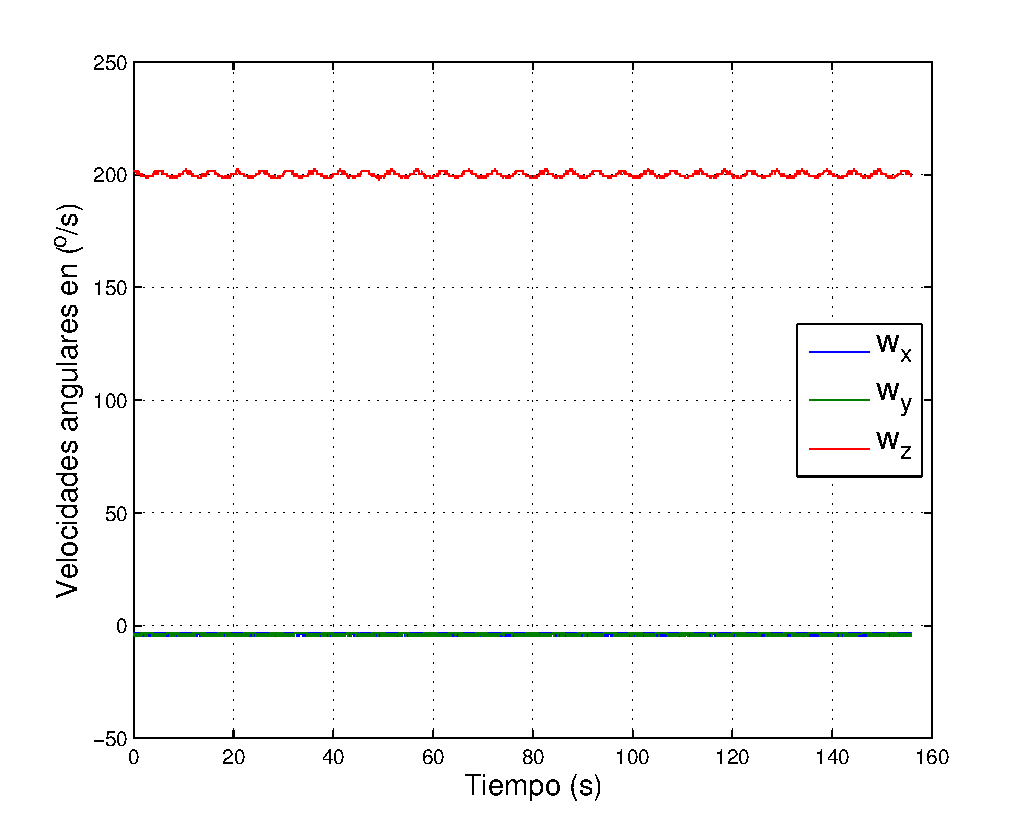
\includegraphics[width=.8\textwidth]{./pics/wcalibradolejos.pdf}
	\caption{Resultados luego de calibrar}
	\label{fig:wcalibradolejos}
\end{figure}

Se puede ver a simple vista que los resultados obtenidos son muy similares a los esperados, obteniendo los siguientes valores promedio:
\begin{table}[H]
\centering
\begin{small}
\begin{tabular}{|c|c|c|}
\hline
\multicolumn{3}{|c|}{\cellcolor[gray]{0.8} \centering \textbf{Aceleración angular ($º/s$)}}\\ \hline
  {\cellcolor[gray]{0.9} \centering \textbf{x}}
& {\cellcolor[gray]{0.9} \centering \textbf{y}}
& {\cellcolor[gray]{0.9} \centering \textbf{z}} \\ \hline  \hline
-3.80 & -3.65 & 200.16 \\ \hline
\end{tabular}
\caption{Resultados ejemplo luego de la calibración}
\label{tab:resultados-ejemplo}
\end{small}
\end{table} 

Es posible notar una oscilación sobre todo en la medida de $w_z$. Dicha oscilación se da a 45 rpm aproximadamente. Si bien no se tiene certeza de su procedencia, es probable que provenga del propio tocadiscos. El mismo posee la posibilidad de girar a 2 velocidades distintas, 33.33rpm (la utilizada) y 45 rpm. Es viable pensar que dentro del tocadiscos hay un solo motor que gira a 45 rpm y se logran los 33.33 rpm mediante una reducción mecánica. De alguna manera el motor podría estar introduciendo una oscilación a su velocidad de giro.\\

Realizando un acercamiento a la velocidad angular obtenida en el eje ``z'' es posible divisar algunos fenómenos interesantes. Analizando la figura \ref{fig:wcalibradocerca} se pueden divisar 2 saltos distintos, como si se contara con 2 resoluciones distintas.

\begin{figure}[h!]
	\centering
	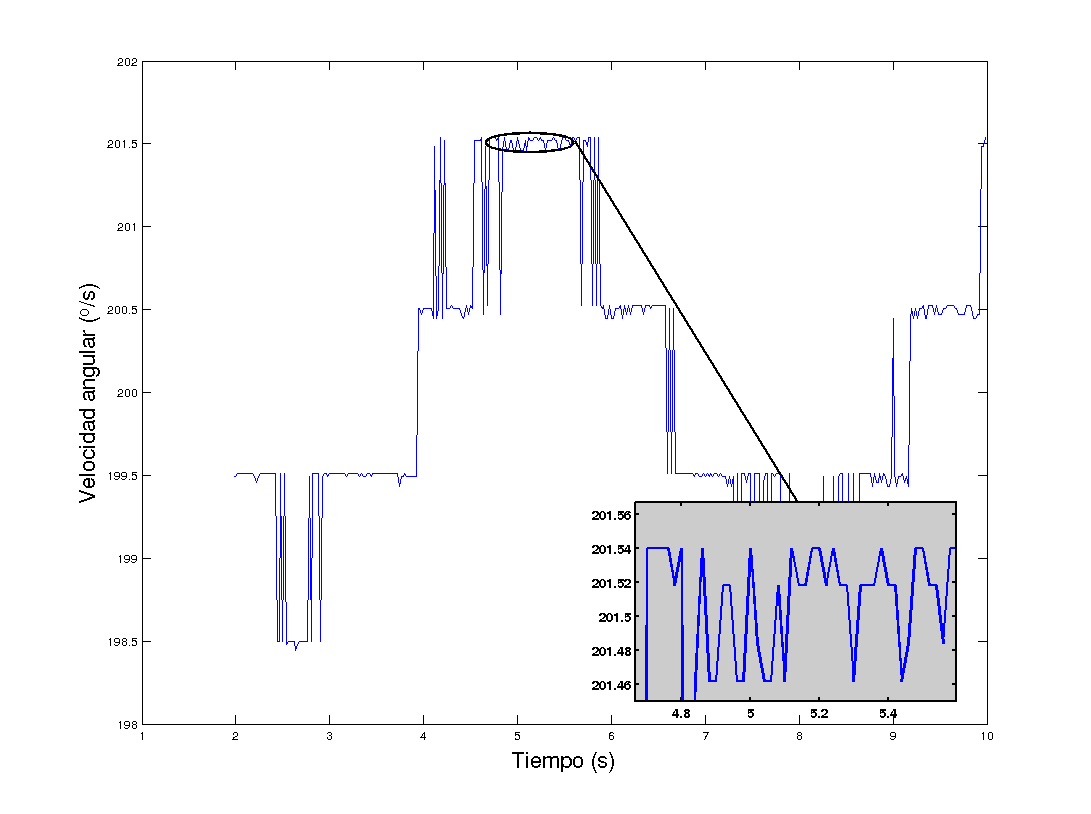
\includegraphics[width=.8\textwidth]{./pics/wcalibradocerca.png}
	\caption{Acercamiento de los resultados luego de calibrar}
	\label{fig:wcalibradocerca}
\end{figure}

Uno de ellos, el más grande, es de aproximadamente $1 º/s$, mientras que el otro, que se observa en el acercamiento realizado en dicha figura, es de aproximadamente $0.05º/s$. Éste último es comparable con el valor hallado de la desviación estándar por lo que puede pensarse como una verificación de la coherencia de los datos obtenidos y calibrados. Por otra parte, los saltos de $1º/s$ no parecen tener, a priori, un sentido claro. Analizando el código que corre internamente en la IMU se detectó el causante de dichos saltos. Resulta que a la hora de enviar los datos, la imu realiza un $cast$ de los valores expresados en punto flotante a entero, lo cual se traduce en una pérdida aberrante de la resolución del instrumento de medida. Es evidente que el código será retocado para evitar esta pérdida de información en el futuro. Por otro lado es importante destacar que este error no afecta al proceso de calibración realizado, ya que se tomaron medidas de velocidades angulares constantes durante todo el tiempo de muestreo y se realizó un promedio de cada tirada, logrando valores más robustos ante dicho fenómeno.

\end{document}